\section{Présentation du port}

\begin{frame}{Le terminal à conteneurs sud}
  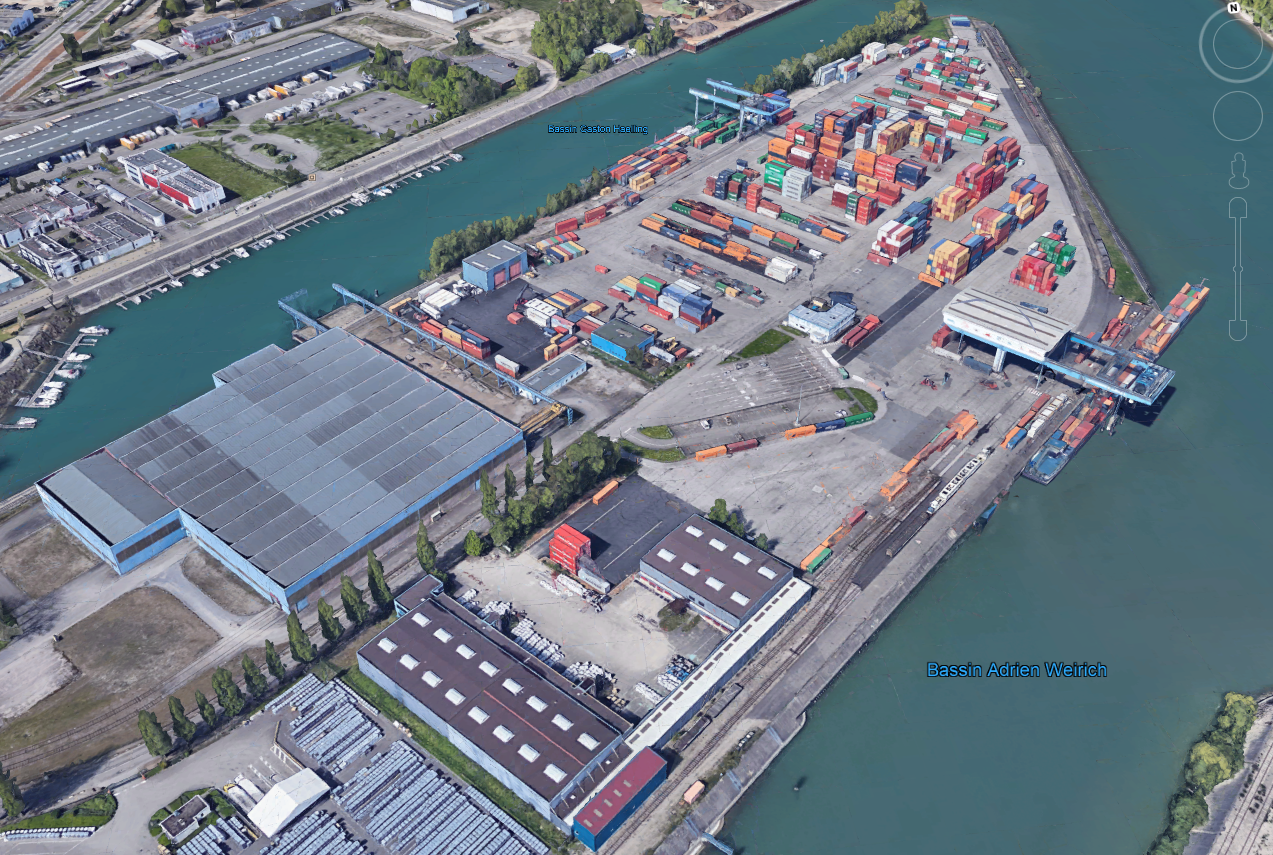
\includegraphics[width=\textwidth]{../images/image14}
\end{frame}

\begin{frame}{Le terminal à conteneurs sud}
  \begin{itemize}
  \item Infrastructures et outillage
    \begin{itemize}
    \item
      2 portiques fluviaux à conteneurs, mobiles
    \item
      1 portique fluvial à colis lourds (capacité 460 tonnes)
    \item
      1 420 mètres de linéaire ferroviaire en 4 voies de longueur variant entre 330 et 400 mètres
    \item
      8 reach-stackers
    \item
      itinéraires routiers adaptés aux colis lourds
    \item
      systèmes informatiques intégrés (TOS)
    \item
      superficie : 10 ha
    \end{itemize}
  \item Enjeux
    \begin{itemize}
    \item Congestion de poids lourds
    \item Elargissement sur un terrain adjacent pour améliorer la fluidité des trafics
    \end{itemize}
  \end{itemize}
\end{frame}

\begin{frame}{Problèmatique du PAS}
  \begin{itemize}
  \item 3000 conteneurs sur le site
  \item 500 entrées/sorties par jour
  \item aucune visibilité sur la date de sortie des conteneurs
  \item politique du First In, First Out
  \end{itemize}
\end{frame}
